\chapter{\vspace{2ex}DASAR TEORITIK, METODOLOGI, DAN PERANCANGAN}

\section{Teori Dasar}
\subsection{Presensi}
Menurut Kamus Besar Bahasa Indonesia (KBBI)~\cite{kbbionline}, presensi diartikan sebagai kehadiran. Kehadiran itu sendiri mengacu pada kehadiran individu atau kelompok di suatu tempat untuk mengikuti acara yang telah direncanakan sebelumnya. Kehadiran karyawan berperan penting dalam menentukan kinerja mereka dalam menyelesaikan tugas~\cite{narulita2024buku}.

\subsection{Aplikasi Presensi}
Aplikasi adalah perangkat lunak yang dirancang untuk menjalankan tugas tertentu pada sistem komputer. Dalam pengembangannya, aplikasi dikategorikan menjadi 3 yaitu aplikasi web, aplikasi \textit{desktop}, dan aplikasi \textit{mobile}.~\cite{pane2020membangun}. Sedangkan, presensi merupakan kehadiran. Maka aplikasi presensi dapat disebut sebagai perangkat lunak yang digunakan untuk mencatat dan memantau kehadiran suatu individu. Menurut Imaniawan dan Rijanandi~\cite{imaniawan2023presensi}, aplikasi presensi memungkinkan pengelolaan data kehadiran secara efisien dikarenakan data dari presensi langsung tersimpan pada server.

\subsection{Lembur}
Menurut Kamus Besar Bahasa Indonesia (KBBI)~\cite{kbbionline}, Lembur merupakan pekerjaan dinas yang dilakukan diluar jam dinas. Berdasarkan Keputusan Menteri Tenaga Kerja Republik Indonesia Nomor KEP. 102 Men VI 2004 pasal 1~\cite{menteri2014peraturan}, perusahaan diwajibkan untuk membayar upah lembur kepada pegawai jika masuk pada kategori berikut:
\begin{enumerate}
    \item Bekerja lebih dari 7 jam dalam sehari atau 40 jam dalam seminggu untuk pegawai yang bekerja selama 6 hari.
    \item Bekerja lebih dari 8 jam sehari dan 40 jam dalam seminggu untuk pegawai yang bekerja selama 5 hari.
    \item Bekerja pada hari istirahat mingguan dan hari libur nasional.
\end{enumerate}

\subsection{\textit{Geolocation}}
Menurut Shellito~\cite{introduction2019bradley}, \textit{Geolocation} adalah teknik yang digunakan untuk menentukan lokasi suatu perangkat di dunia nyata, seperti \textit{smartphone}, tablet, atau komputer. Dengan \textit{Geolocation}, perangkat dapat mengetahui koordinatnya (lintang dan bujur) melalui berbagai metode, seperti alamat IP, koneksi Wi-Fi, menara seluler, atau GPS. Setelah lokasi ditentukan, informasi tersebut dapat dipetakan dan dibagikan melalui internet.

\subsection{Haversine}
Haversine merupakan metode paling populer yang menggunakan trigonometri untuk menghitung jarak lingkaran besar dengan menggunakan koordinat yang didefinisikan dalam derajat desimal sebagai \textit{input}. Rumus Haversine adalah rumus pengukuran jarak yang paling umum digunakan karena relatif ringan dari segi pengkodean dan cukup akurat dalam kebanyakan kasus~\cite{learning2019joel}. Menurut Xiao~\cite{gis2015xiao}, langkah pertama pada rumus Haversine yaitu mencari nilai a atau nilai antara yang dapat dilihat pada \textbf{Persamaan \ref{eq:nilai-a}}.
\begin{equation}
    a = \sin^2 \left( \frac{d\varphi}{2} \right) + \cos(\varphi_1) \cdot \cos(\varphi_2) \cdot \sin^2 \left( \frac{d\lambda}{2} \right)
\label{eq:nilai-a}
\end{equation}


\noindent Keterangan:
\\
$d\varphi$ = Perbedaan lintang antara dua titik ($\varphi_2 - \varphi_1$).
\\
$\varphi_1$ = Lintang titik pertama (dalam radian).
\\
$\varphi_2$ = Lintang titik kedua (dalam radian).
\\
$d\lambda$ = Perbedaan bujur antara dua titik ($\lambda_2 - \lambda_1$).
\\
$\lambda_1$ = Bujur titik pertama (dalam radian).
\\
$\lambda_2$ = Bujur titik kedua (dalam radian).
\\

Selanjutnya, mencari nilai c atau jarak sudut antara dua titik pada permukaan bola dalam radian menggunakan nilai a yang sudah didapatkan sebelumnya yang dapat dilihat pada \textbf{Persamaan \ref{eq:nilai-c}}.
\begin{equation}
    c = 2 \, \text{arcsin} \left( \min(1, \sqrt{a}) \right)
\label{eq:nilai-c}
\end{equation}

Setelah itu, mencari nilai d atau jarak sebenarnya antara dua titik dalam permukaan bumi dengan mengalikan nilai jarak sudut (c) dengan jari-jari bumi (6371 km) yang dapat dilihat pada \textbf{Persamaan \ref{eq:nilai-d}}.
\begin{equation}
    d = cR
\label{eq:nilai-d}
\end{equation}

Berikut ini adalah contoh perhitungan manual menggunakan rumus Haversine antara titik koordinat Universitas Tarumanagara (-6.19058187063816, 106.79779495106814) dengan titik koordinat MyPassword (-6.169336170685656, 106.78859045462738). Langkah pertama adalah melakukan konversi lintang dan bujur kedua titik menjadi radian dan mencari nilai perbedaan lintang dan bujur antara dua titik.
\\
$\varphi_1 = -6,19058187063816 \cdot \left( \frac{\pi}{180} \right) = -0.10804603626 $ radian 
\\
$\lambda_1 = 106,79779495106814 \cdot \left( \frac{\pi}{180} \right) = 1,86397315577 $ radian
\\
$\varphi_2 = -6,169336170685656 \cdot \left( \frac{\pi}{180} \right) = -0,10767522884 $ radian
\\
$\lambda_2 = 106,78859045462738 \cdot \left( \frac{\pi}{180} \right) = 1,86381250700 $ radian
\\
$d\varphi = -0,10767522884 - (-0,10804603626) = 0,00037080742 $ radian
\\
$d\lambda = 1,86381250700 - 1,86397315577 = -0,00016064877 $ radian
\\


Setelah melakukan pengubahan semua lintang dan bujur menjadi radian. Selanjutnya, melakukan perhitungan untuk mencari nilai $c$ atau jarak sudut antara dua titik.
\\
$a = \sin^2 \left( \frac{0,00037080742}{2} \right) + \cos(-0.10804603626) \cdot \cos(-0,10767522884) \cdot \sin^2 \left( \frac{-0,00016064877}{2} \right)$
\\
$a = (0,0001854037)^2 + 0,99416870319 \cdot 0,9942086212 \cdot  (-0,00008032438)^2 $
\\
$a = 3,4374535 $ x $10^-8$ + $0,99416870319 \cdot 0,9942086212 \cdot 6,452007$ x $10^-9 $
\\
$a = 4,0751770 $ x $ 10^-8 $
\\


Selanjutnya menghitung nilai c atau jarak sudut antara dua titik menggunakan nilai a atau nilai antara yang sudah didapatkan sebelumnya.
\\
$c = 2 \cdot \, \text{arcsin} \left( \min(1, \sqrt{4,0751770 \, \text{x} \, 10^-8}) \right)$
\\
$c = 2 \cdot \, \text{arcsin} \, 0,00020187066 $
\\
$c = 0,00040374135 $
\\

Terakhir, menghitung jarak dua titik dalam permukaan bumi menggunakan nilai c atau jarak sudut antara dua titik dengan jari-jari bumi (6371 km).
\\
$d = 0,00040374135 \cdot 6371 $
\\
$d = 2,5722361635632 $
\\


Jadi, hasil jarak yang dihitung antara Universitas Tarumanagara dan MyPassword menggunakan rumus Haversine adalah 2,57 km.



\subsection{\textit{World Wide Web} atau Web}
\textit{World Wide Web} (WWW) atau Web adalah sebuah aplikasi perangkat lunak yang memudahkan dan memungkinkan hampir semua orang untuk menerbitkan dan menjelajahi dokumen \textit{hypertext} pada internet~\cite{zero2022jain}. Web menggunakan protokol HTTP, yang merupakan salah satu dari sekian banyak bahasa yang digunakan di Internet untuk mengirimkan data. Web juga memanfaatkan \textit{browser} seperti \textit{Internet Explorer} atau \textit{Firefox} untuk membuka dokumen Web yang dikenal sebagai halaman Web. Halaman-halaman ini terhubung satu sama lain melalui \textit{hyperlink}. Dokumen \textit{Web} dapat berisi grafik, suara, teks, dan video~\cite{sastradipraja2022konsep}.

\subsection{\textit{Website}}
\textit{Website} adalah media dengan banyak halaman yang saling terhubung (\textit{hyperlink}) dan berfungsi untuk memberikan informasi dalam bentuk teks, gambar, video, suara, dan animasi. \textit{Website} modern umumnya bersifat dinamis, sedangkan \textit{website} statis kini jarang ditemukan. Halaman-halaman pada \textit{website} terhubung dan diakses melalui \textit{domain} (URL) di \textit{World Wide Web} (WWW), serta menggunakan \textit{hosting} untuk menyimpan data. \textit{Website} diakses menggunakan \textit{browser} seperti \textit{Chrome, Mozilla Firefox, Internet Explorer} (IE), dan \textit{Opera}~\cite{2020buku}. Menurut Asari \textit{et al}.~\cite{andipengembangan}, \textit{website} dibagi menjadi 2 yaitu \textit{web} dinamis yang merupakan \textit{web} tanpa \textit{database} dikarenakan isi \textit{web} tersebut tidak akan berubah informasinya, sedangkan \textit{web} dinamis merupakan \textit{web} yang isi halamannya selalu berubah secara berkala. Contoh \textit{website} dapat dilihat pada \textbf{\ref{fig:contoh-website}}.
%
\begin{figure}[!htbp]
	\centering
	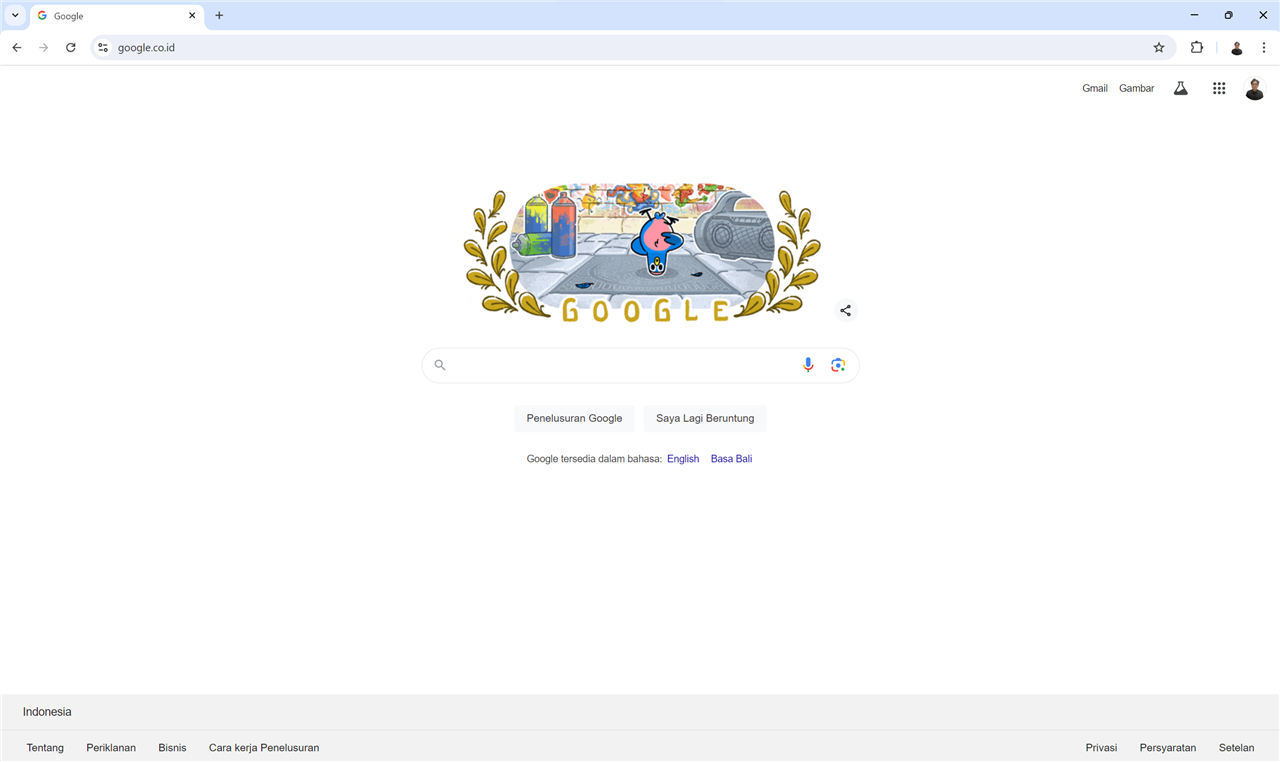
\includegraphics[width=10cm]{Gambar/bab2/website.png}
	\caption{Contoh \textit{Website}~\cite{website2024google}}
	\label{fig:contoh-website}
\end{figure}
\FloatBarrier
%
\subsection{\textit{Web Page}}
Menurut Kumar~\cite{web2018akshi}, \textit{Web page} merupakan dokumen yang ditampilkan pada \textit{web browser}. \textit{Web page} bisa bersifat statis atau dinamis. Statis berarti halaman tersebut tetap sama atau tidak berubah, sementara dinamis berarti halaman tersebut dapat berubah. Oleh karena itu, halaman web statis berisi konten yang sama setiap kali halaman dimuat, sedangkan konten halaman web dinamis dapat dihasilkan secara langsung saat dibutuhkan. Pada \textbf{\ref{fig:contoh-web-page}} merupakan contoh \textit{web page} dengan url \url{https://www.microsoft.com/id-id/microsoft-365} yang merupakan bagian satu halaman dari \textit{website} \url{https://www.microsoft.com/id-id/}.
%
\begin{figure}[!htbp]
	\centering
	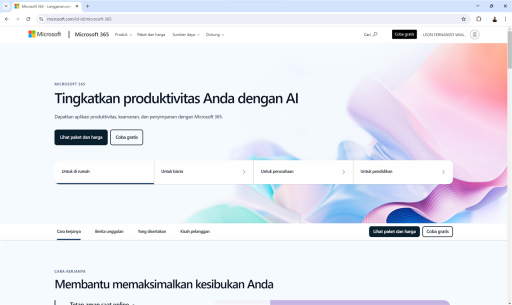
\includegraphics[width=10cm]{Gambar/bab2/web-page.png}
	\caption{Contoh \textit{Web Page}~\cite{webpage2024microsoft}}
	\label{fig:contoh-web-page}
\end{figure}
\FloatBarrier
%

\subsection{\textit{Scrum}}
Scrum adalah kerangka kerja yang dirancang untuk menerapkan prinsip-prinsip Agile dalam pengembangan. Konsep Scrum pertama kali diperkenalkan dalam artikel berjudul "The New New Product Development Game" oleh Takeuchi dan Nonaka, yang diterbitkan oleh Harvard Business Review (HBR) pada tahun 1986~\cite{magdalena2023scrum}. Menurut Hooda dkk.~\cite{hooda2023agile}, \textit{Scrum} terdiri dari 3 tahap utama yaitu \textit{outline planning}, \textit{sprint cycle}, dan \textit{project closure} yang dapat dilihat pada \textbf{\ref{fig:scrum-phases}}.
\begin{enumerate}
    \item \textit{Outline Planning}
    \\
    Pada tahap pertama, penulis akan melakukan analisis dan identifikasi kebutuhan pengguna untuk perangkat lunak. Pada tahap ini, \textit{product backlog} juga disusun, berisi daftar fitur yang dibutuhkan oleh perangkat lunak, yang diurutkan berdasarkan prioritas.
    
    \item \textit{Sprint Cycle}
    \\
    Pada tahap ini, \textit{sprint} dimulai dengan \textit{sprint planning}, yaitu proses pemilihan item dari \textit{product backlog} yang akan dikerjakan dalam setiap \textit{sprint}. Setiap \textit{sprint} berlangsung dalam iterasi pendek yang biasanya berkisar antara 1 hingga 4 minggu. Pada iterasi ini akan berfokus pada penyelesaian \textit{item} yang telah dipilih. Pada akhir setiap \textit{sprint} akan dilakukan \textit{sprint review} untuk memastikan bahwa item yang dikerjakan sudah sesuai memenuhi kriteria yang diharapkan. Siklus sprint ini akan terus berulang sampai semua item pada \textit{product backlog} terselesaikan atau proyek sudah mencapai tujuannya.

    \item \textit{Project Closure}
    \\
    Tahap terakhir adalah fase penutupan, di mana proyek diselesaikan dan ditutup secara resmi. Aktivitas yang dilakukan di tahap ini mencakup penyelesaian dokumentasi yang diperlukan, seperti panduan sistem atau manual pengguna.
\end{enumerate}
%
\begin{figure}[!htbp]
	\centering
	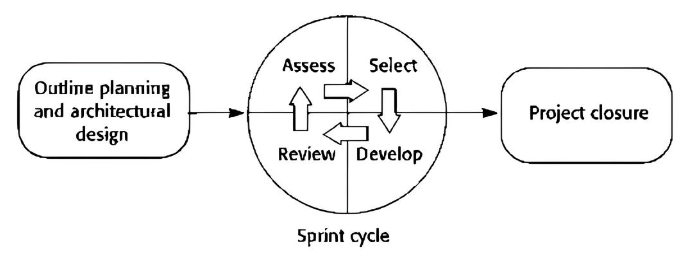
\includegraphics[width=10cm]{Gambar/bab2/scrum-methodology.png}
	\caption{\textit{Scrum Phases}~\cite{sommerville2014software}}
	\label{fig:scrum-phases}
\end{figure}
\FloatBarrier
%
Menurut Pagotto~\cite{7521555}, Metode \textit{scrum} dapat dilakukan secara individu atau sendiri yang disebut sebagai \textit{scrum solo}. \textit{Scrum Solo} memiliki karakteristik mirip dengan \textit{scrum}, seperti \textit{backlog} produk dan \textit{sprint}. Namun, \textit{scrum Solo} menggunakan \textit{sprint} satu minggu tanpa pertemuan harian. Di akhir setiap \textit{sprint}, pengembang harus menyampaikan prototipe perangkat lunak baru, dan pertemuan dengan klien atau pengguna akhir dilakukan jika diperlukan. \textit{Scrum Solo} mengintegrasikan praktik baik dari \textit{scrum} dengan fleksibilitas tambahan. Berikut ini adalah beberapa aktor proses untuk pengembangan secara individu:
\begin{enumerate}
    \item \textit{Product Owner}
    \\
    Pemilik produk yang bertanggung jawab atas visi dan arah dari produk, berinteraksi langsung dengan produk, baik sebagai individu atau sekelompok pengguna serta memastikan bahwa produk memenuhi kebutuhan pengguna dan tujuan bisnis. Mereka memberikan arahan dan keputusan penting tentang fitur dan prioritas produk.

    \item \textit{Individual Developer}
    \\
    Pengembang individu yang bertanggung jawab untuk menjalankan proses pengembangan dan membangun produk. Memiliki peran menulis kode, mengimplementasikan fitur, memperbaiki bug, dan memastikan bahwa produk berfungsi dengan baik. \textit{Individual Developer} memiliki tanggung jawab mengikuti spesifikasi dan arahan yang diberikan oleh \textit{Product Owner}, dan memastikan bahwa produk dikembangkan sesuai dengan standar dan tenggat waktu yang ditetapkan.

    \item \textit{Advisor}
    \\
     Konsultan yang memiliki pengetahuan mendalam tentang proses pengembangan. \textit{Advisor} memiliki peran Memberikan saran dan panduan tentang teknologi yang digunakan dan cakupan proyek dan bertanggung jawab menyediakan wawasan luas tentang teknologi dan metodologi yang digunakan dalam pengembangan produk, serta membantu tim dalam mengatasi tantangan teknis dan strategis.

     \item \textit{Validation Group}
     \\
     Pengguna potensial dari produk yang dihasilkan. \textit{Validation Group} memiliki peran berpartisipasi dalam proses validasi produk, dan tanggung jawab menguji produk dan memberikan umpan balik untuk memastikan bahwa produk memenuhi kebutuhan dan ekspektasi pengguna. Partisipasi mereka harus didokumentasikan dalam laporan proses.
    
\end{enumerate}

\subsection{PT Password Solusi Sistem}
Berdasarkan \textit{web} resmi MyPassword~\cite{aboutuswebsite}, MyPassword didirikan pada tahun 2009 sebagai perusahaan solusi teknologi informasi dan integrator sistem, yang menyediakan solusi infrastruktur teknologi informasi dan aplikasi bisnis, termasuk memberikan implementasi, pemeliharaan, dan layanan lainnya. Perusahaan ini dipimpin oleh dua direktur yaitu Bapak Hendriyanto Suhandi dan Bapak Julius Wendra Lea. Logo MyPassword dapat dilihat pada \textbf{\ref{fig:logo-mypassword}}.
%
\begin{figure}[!htbp]
	\centering
	
\includegraphics[width=10cm]{Gambar/bab2/logo-mypassword.png}
	\caption{Logo MyPassword~\cite{aboutuswebsite}}
	\label{fig:logo-mypassword}
\end{figure}
\FloatBarrier
%
Kantor MyPassword berlokasi di Wisma 77 \textit{Tower} 1, Lantai 15 yang dapat dilihat pada \textbf{\ref{fig:gedung-wisma-77}}, dengan alamat di Jl. Letjen S. Parman No.Kav. 77, RT.6/RW.3, Slipi, Kecamatan Palmerah, Kota Jakarta Barat, Daerah Khusus Ibukota Jakarta, 11410. MyPassword menyediakan beberapa solusi dan layanan yang ditawarkan diantaranya \textit{Modern Data Center, Modern Information System, Modern Office}, dan \textit{Modern Services}.
%
\begin{figure}[!htbp]
	\centering
	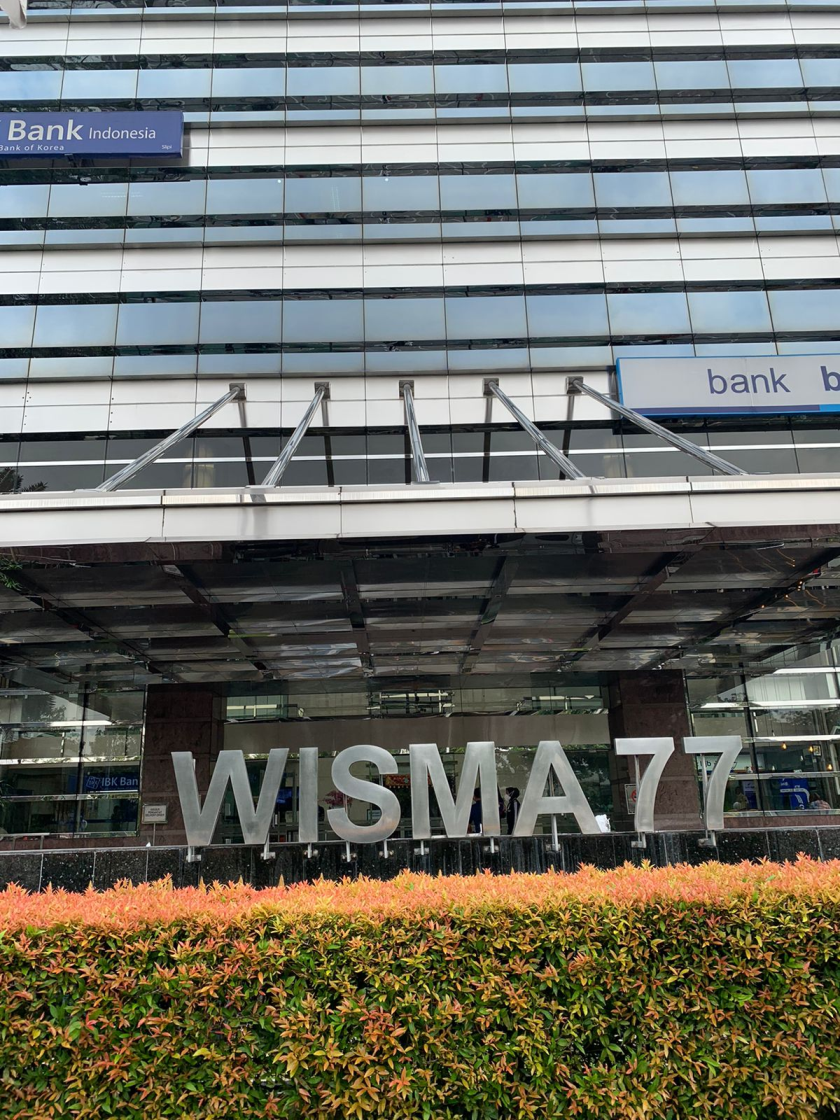
\includegraphics[width=5cm]{Gambar/bab2/gedung-wisma-77.jpeg}
	\caption{Gedung Wisma 77 \textit{Tower} 1}
	\label{fig:gedung-wisma-77}
\end{figure}
\FloatBarrier
%
MyPassword terdiri dari beberapa divisi diantaranya yaitu \textit{Business Application, Human Resources, Infrastructure, Business Support,} dan lain-lain. Jam kerja utama di kantor MyPassword yaitu Senin sampai Jumat, mulai pukul 8 pagi hingga 5 sore. Namun, untuk divisi \textit{Infrastructure} tidak semua \textit{staff} menggunakan jam kerja utama, tetapi \textit{staff Infrastructure} bekerja menggunakan jam \textit{shift} yang sudah ditentukan sehingga jam kerja mungkin akan berbeda antara satu \textit{staff} dengan \textit{staff} lainnya. Selanjutnya pada kantor MyPassword terdapat kerja lembur salah satunya divisi \textit{Infrastructure}, yang bekerja diluar jam \textit{shift} yang telah ditentukan atau bekerja pada hari libur nasional. Kerja lembur pada MyPassword juga tidak hanya dilakukan di kantor saja, tetapi juga bisa dilaksanakan di luar kantor.

Saat ini pencatatan lembur pada MyPassword sudah menggunakan aplikasi bernama "Andal". Aplikasi ini dibeli melalui pihak eksternal dengan \textit{one time payment}. Aplikasi ini dapat di-\textit{download} melalui \textit{playstore} ataupun \textit{appstore}. Pada proses bisnis aplikasi ini, \textit{Staff Infrastructure} harus melakukan presensi terlebih dahulu sebelum melakukan pengajuan lembur. Saat presensi akan dilakukan pengambilan lokasi dan foto \textit{Staff Infrastructure}. Setelah melakukan presensi maka \textit{Staff Infrastructure} dapat mengajukan formulir lembur yang mengacu pada presensi yang telah dilakukan. Jika \textit{Staff Infrastructure} lupa melakukan presensi pada hari kerja lembur maka tidak bisa melakukan pengajuan lembur sehingga \textit{Staff Infrastructure} perlu mengajukan \textit{form attendance correction} pada aplikasi. Permasalahan utama dari aplikasi yang saat ini digunakan adalah kurangnya fleksibilitas dalam penyesuaian, karena fitur-fiturnya sudah ditentukan berdasarkan layanan dari pihak ketiga. Akibatnya, ketika \textit{Staff Infrastructure} melakukan lembur lebih dari satu kali dalam sehari dalam aplikasi, perhitungan lembur harus dilakukan secara manual, yang mengakibatkan proses menjadi tidak efisien.








\section{Perancangan Proses}
Pada fase ini, akan dilakukan wawancara dengan Ibu Melissa selaku \textit{Manager Human Resource} di MyPassword. Wawancara ini akan membahas fitur-fitur yang diperlukan pada aplikasi yang akan dikembangkan dan cara pencatatan data lembur saat ini. Selain itu, wawancara ini juga akan mengeksplorasi tantangan yang dihadapi dengan menggunakan cara pencatatan lembur saat ini. \textbf{\ref{fig:wawancara-manager-human-resources}} menunjukkan sesi wawancara dengan \textit{Manager Human Resources} secara langsung di kantor MyPassword pada tanggal 26 Juli 2024 sekitar pukul 12 siang. Hasil dari wawancara dapat ditemukan pada \hyperref[sec:wawancara]{\textbf{Lampiran~II}}.

\begin{figure}[!htbp]
	\centering
	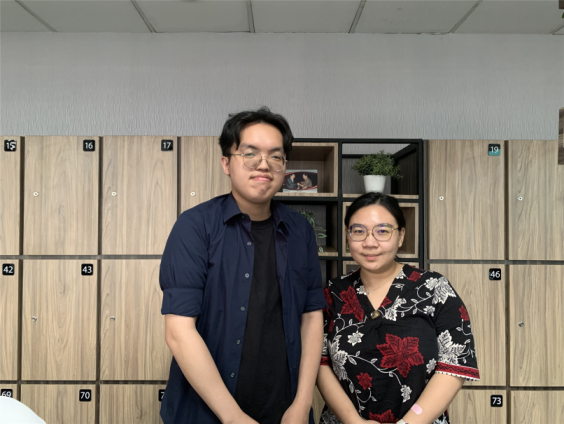
\includegraphics[width=7cm]{Gambar/bab2/dokumentasi-wawancara.jpg}
	\caption{Wawancara bersama \textit{Manager Human Resources} MyPassword}
	\label{fig:wawancara-manager-human-resources}
\end{figure}
\FloatBarrier

\subsection{Teori Umum}
\subsubsection{UML}
UML (\textit{Unified Modeling Language}) adalah bahasa grafis untuk menentukan, memvisualisasikan, membangun, dan mendokumentasikan artefak dari sistem perangkat lunak. Alat ini membantu dalam pemahaman yang lebih baik tentang perangkat lunak atau sistem atau produk yang akan dikembangkan, baik di antara pengembang maupun pelanggan~\cite{uml2022suriya}. Menurut Unhelkar~\cite{unhelkar2017software}, UML juga dapat membantu memodelkan persyaratan sistem baru dan membantu memahami proses bisnis dan aplikasi yang ada. Unhelkar juga menjelaskan terdapat beberapa jenis-jenis diagram UML:
\begin{enumerate}
    \item \textit{Use Case Diagram}
    \\ Memberikan gambaran umum tentang fungsionalitas sistem atau proses bisnis dari perspektif pengguna. Cara pengguna “menggunakan” sistem adalah titik awal untuk membuat diagram \textit{use case}.

    \item \textit{Activity Diagram}
    \\ Memodelkan aliran aktivitas normal dalam sistem dan alternatif serta pengecualian yang sangat baik digambarkan oleh diagram ini di mana saja interaksi terjadi. Khususnya, aliran dalam model \textit{use case} ke \textit{use case} di bawah diagram.

    \item \textit{Class Diagram}
    \\ Mewakili kelas, definisi mereka, hubungan, kelas dan entitas dari ruang masalah adalah entitas teknis terperinci di ruang solusi. Atribut dan operasi yang mendefinisikan kelas termasuk dalam diagram kelas ini. Hubungan dalam diagram kelas menggambarkan bagaimana kelas berinteraksi, berkolaborasi, dan mewarisi dari kelas lain.

    \item \textit{Sequence Diagram}
    \\ Memodelkan interaksi antar objek berdasarkan garis waktu mereka. Objek dapat berupa tabel, antarmuka pengguna, dan pengendali atau kelas lain juga dapat mewakili relasional untuk secara khusus ditunjukkan pada diagram ini atau mereka dapat menjadi objek anonim yang termasuk dalam suatu kelas. Urutan eksekusi pesan antar objek pada waktu runtime dimodelkan dengan baik oleh diagram ini, oleh karena itu namanya.
\end{enumerate}

\subsection{Gambar Diagram Rancangan Proses}
\subsubsection{\textit{Use Case Diagram}}
Pada rancangan \textit{use case diagram} untuk aplikasi presensi terdiri dari 3 aktor yaitu: (i) \textit{staff Infrastructure} dapat melakukan presensi masuk dan presensi keluar, serta melakukan pengajuan lembur, (ii) \textit{Manager Infrastructure} memiliki tugas untuk melakukan \textit{reject} atau \textit{penolakkan} pada data lembur yang tidak \textit{valid} dan melihat laporan lembur dan presensi (iii) \textit{Manager Human Resources} yang bertugas mengelola akun \textit{user}, melihat laporan data presensi dan lembur. \textit{Use case diagram} dari perancangan aplikasi presensi \textit{online} berbasis \textit{web} pada PT Password Solusi Sistem dapat dilihat pada \hyperref[sec:use-case-diagram-aplikasi-presensi-online]{\textbf{Lampiran~III}}.

Pada aplikasi presensi \textit{online}, \textit{staff Infrastructure} dapat melakukan \textit{login} dan \textit{logout} pada sistem, jika tidak memiliki akun dapat melakukan registrasi. \textit{Staff Infrastructure} dapat melihat jadwal jam kerja dan melakukan presensi masuk atau keluar, setelah itu mengaktifkan akses kamera dan lokasi, jika \textit{staff Infrastructure} melakukan presensi diluar jam \textit{shift} atau libur perusahaan maka sistem akan mengecek berdasarkan data \textit{shift} jam kerja \textit{staff Infrastructure} dan data hari libur perusahaan, jika syarat terpenuhi maka akan mencatat jam lembur tersebut. \textit{Staff Infrastructure} dapat melihat data riwayat presensi dan lembur, serta mengajukan \textit{form overtime request correction} jika \textit{staff Infrastructure} lupa melakukan presensi lembur. \textit{Manager Infrastructure} dan \textit{Manager Human Resource} memiliki beberapa akses yang sama seperti melakukan \textit{login} dan \textit{logout}, melihat data presensi dan lembur seluruh \textit{staff Infrastructure}, melakukan \textit{export} data presensi dan lembur dalam bentuk \textit{Microsoft Excel}, mengelola akun \textit{user} yang telah registrasi seperti mengaktifkan atau menonaktifkan, mengelola data hari libur perusahaan, mengelola \textit{shift} jam kerja \textit{staff Infrastructure} yang akan digunakan untuk pengecekkan presensi lembur. Selanjutnya perbedaan tambahan pada \textit{Manager Infrastructure} yaitu harus melakukan registrasi akun pada awal dan dapat melakukan penolakkan atau \textit{reject} pada data lembur \textit{Staff Infrastructure} yang tidak \textit{valid}.


\subsubsection{\textit{Use Case Scenario}}
\textit{Use case scenario} pada perancangan aplikasi presensi \textit{online} berbasis \textit{web} pada PT Password Solusi Sistem dapat dilihat pada \hyperref[sec:use-case-scenario-aplikasi-presensi-online]{\textbf{Lampiran~IV}}.

\subsubsection{\textit{Activity Diagram}}
\textit{Activity diagram} dari perancangan aplikasi presensi \textit{online} berbasis \textit{web} pada PT Password Solusi Sistem dapat dilihat pada \hyperref[sec:activity-diagram-aplikasi-presensi-online]{\textbf{Lampiran~V}}.

\subsubsection{\textit{Sequence Diagram}}
\textit{Sequence diagram} dari perancangan aplikasi presensi \textit{online} berbasis \textit{web} pada PT Password Solusi Sistem dapat dilihat pada \hyperref[sec:sequence-diagram-aplikasi-presensi-online]{\textbf{Lampiran~VI}}.

\subsubsection{\textit{Class Diagram}}
\textit{Class diagram} dari perancangan aplikasi presensi \textit{online} berbasis \textit{web} pada PT Password Solusi Sistem dapat dilihat pada \hyperref[sec:class-diagram-aplikasi-presensi-online]{\textbf{Lampiran~VII}}.

\section{Perancangan Basis Data}
Basis data didefinisikan sebagai kumpulan informasi yang terorganisir dan saling terkait. Tujuan utama basis data adalah untuk mengelola sejumlah besar data yang disimpan dan menyediakan informasi darinya~\cite{database2022jagdish}. Desain basis data adalah proses menghasilkan model data yang terperinci dari sebuah basis data~\cite{database2019date}. Model data \textit{entity-relationship} (E-R) adalah model data yang banyak digunakan untuk desain basis data. Model ini menyediakan representasi grafis yang nyaman untuk melihat data, hubungan, dan batasan~\cite{database2019abraham}. Menurut Conolly dan Begg~\cite{conolly2015database}, terdapat tiga fase dalam desain basis data yaitu \textit{conceptual database design, logical database design,} dan \textit{physical database design}.


\subsection{\textit{Conceptual Database Design}}
\textit{Conceptual data design} merupakan tahap untuk membangun representasi konseptual dari basis data, yang meliputi identifikasi entitas, hubungan, dan atribut penting~\cite{conolly2015database}. Perancangan \textit{conceptual data modeling} akan dilakukan dengan mengindentifikasi \textit{entity} berdasarkan hasil wawancara dengan \textit{Manager Human Resouces} di PT Password Solusi Sistem. Pada \textbf{\ref{tab:indentifikasi-entity}} menunjukkan hasil identifikasi \textit{entity} berdasarkan kebutuhan MyPassword. Pada \textbf{\ref{tab:indentifikasi-hubungan-antar-entity}} menunjukkan hubungan antar \textit{entity}. \textit{Conceptual data modeling} dalam bentuk diagram dapat dilihat pada \hyperref[sec:conceptual-database-design]{\textbf{Lampiran~VIII}}.
%%%%%%%%%%%%%%%%%%%%%%%%%%%%%%%%%%%%%%%%%%%%%%%%%%%%%%%%%%%%%%%%%
\FloatBarrier
\begin{longtable}{ |p{3cm}|p{6cm}|p{6cm}|}
\caption{Identifikasi \textit{Entity}}\label{tab:indentifikasi-entity} 
\\
\hline
\textbf{\textit{Entity}}
&\textbf{Deskripsi}
&\textbf{Kejadian / Kemunculan}
\\ 
\hline

\textit{User}
&Informasi tentang \textit{user} pada aplikasi presensi \textit{online}.
&Data \textit{user} akan dibuat ketika \textit{Staff} atau \textit{Manager Infrastructure} melakukan registrasi.
\\ 
\hline

\textit{Shift}
&Informasi tentang jenis \textit{shift} kerja.
&Data \textit{Shift} ditambahkan oleh \textit{Manager Human Resources} dan \textit{Manager Infrastructure}.
\\ 
\hline

\textit{ShiftDay}
&Informasi tentang hari dan waktu spesifik dari setiap jenis \textit{shift} yang akan digunakan untuk perhitungan lembur.
&Data \textit{ShiftDay} ditambahkan oleh \textit{Manager Human Resources} dan \textit{Manager Infrastructure}.
\\ 
\hline

\textit{Holiday}
&Informasi tentang jenis libur perusahaan.
&Data \textit{Holiday} ditambahkan oleh \textit{Manager Human Resources} dan \textit{Manager Infrastructure}.
\\ 
\hline

\textit{HolidayDay}
&Informasi tentang hari dan waktu spesifik dari setiap jenis \textit{holiday} yang akan digunakan untuk perhitungan lembur.
&Data \textit{HolidayDay} ditambahkan oleh \textit{Manager Human Resources} dan \textit{Manager Infrastructure}.
\\ 
\hline

\textit{Department}
&Informasi tentang divisi dari setiap \textit{user}.
&Data \textit{Department} ditambahkan oleh \textit{Manager Human Resources} dan \textit{Manager Infrastructure}.
\\ 
\hline

\textit{Role}
&Informasi tentang jabatan dari setiap \textit{user}.
&Data \textit{Role} ditambahkan oleh \textit{Manager Human Resources} dan \textit{Manager Infrastructure}.
\\ 
\hline

\textit{Attendance}
&Informasi tentang presensi setiap \textit{user} yang akan digunakan untuk perhitungan lembur.
&Data \textit{Attendance} akan ditambahkan ketika \textit{staff Infrastructure} melakukan presensi.
\\ 
\hline

\textit{Overtime}
&Informasi tentang lembur dari setiap \textit{staff Infrastructure}.
&Data \textit{Overtime} akan ditambahkan secara otomatis jika \textit{staff Infrastructure} melakukan presensi diluar jam \textit{shift} ataupun pada hari libur. Data \textit{Overtime} juga dapat ditambahkan secara manual oleh \textit{staff Infrastructure}.
\\ 
\hline

\textit{Session}
&Informasi tentang \textit{Session} setiap \textit{user}.
&Data \textit{Session} akan diregenerasi secara otomatis ketika \textit{user} melakukan \textit{login}.
\\
\hline

\textit{ActivityType}
&Informasi tentang jenis kerja yang dilakukan oleh \textit{staff} seperti WFO, WFH atau \textit{remote}.
&Data \textit{ActivityType} ditambahkan secara \textit{default} dengan nilai yang telah ditentukan.
\\
\hline

\textit{ActivityCategory}
&Informasi tentang kategori aktivitas pekerjaan yang dilakukan oleh \textit{staff Infrastructure} seperti instalasi dan sebagainya.
&Data \textit{ActivityCategory} ditambahkan secara \textit{default} dengan nilai yang telah ditentukan.
\\
\hline

\textit{ShiftScheduling}
&Informasi tentang penjadwalan \textit{shift} yang akan digunakan oleh setiap \textit{staff} berdasarkan jangka waktu yang diatur.
&Data \textit{ShiftScheduling} ditambahkan oleh \textit{Manager Human Resources} dan \textit{Manager Infrastructure}.
\\
\hline

\end{longtable}


%%%%%%%%%%%%%%%%%%%%%%%%%%%%%%%%%%%%%%%%%%%%%%%%%%%%%%%%%%%%%%%%%
\FloatBarrier
\begin{longtable}{ |p{2cm}|p{3cm}|p{3cm}|p{3cm}|p{3cm}|}
\caption{Identifikasi Hubungan Antar \textit{Entity}}\label{tab:indentifikasi-hubungan-antar-entity} 
\\
\hline
\textbf{\textit{Entity}}
&\textbf{\textit{Multiplicity}}
&\textbf{\textit{Relationship}}
&\textbf{\textit{Multiplicity}}
&\textbf{\textit{Entity}}
\\ 
\hline

\multirow{2}{*}{\textit{Shift}}
&1..1
&\textit{AssignedOn}
&1..*
&\textit{ShiftDay}
\\ 
\cline{2-5}
&1..1
&\textit{ShiftAssignments}
&0..*
&\textit{ShiftScheduling}
\\ 
\hline

\multirow{3}{*}{\textit{Attendance}}
&0..1
&\textit{Includes}
&0..1
&\textit{Overtime}
\\
\cline{2-5}
&1..*
&\textit{CategorizedBy}
&1..1
&\textit{ActivityType}
\\ 
\cline{2-5}
&1..*
&\textit{ClassifiedAs}
&1..1
&\textit{ActivityCategory}
\\ 
\hline

\multirow{8}{*}{\textit{User}}
&1..*
&\textit{WorksIn}
&1..1
&\textit{Department}
\\
\cline{2-5}
&1..*
&\textit{AssignedAs}
&1..1
&\textit{Role}
\\ 
\cline{2-5}
&1..1
&\textit{Records}
&0..*
&\textit{Attendance}
\\ 
\cline{2-5}
&0..1
&\textit{Requests}
&0..*
&\textit{Overtime}
\\ 
\cline{2-5}
&1..*
&\textit{ScheduledFor}
&0..1
&\textit{Shift}
\\ 
\cline{2-5}
&1..1
&\textit{Attends}
&1..1
&\textit{Session}
\\ 
\cline{2-5}
&1..*
&\textit{EntitledTo}
&0..1
&\textit{Holiday}
\\ 
\cline{2-5}
&1..1
&\textit{HasSchedules}
&0..*
&\textit{ShiftScheduling}
\\ 
\hline

\textit{Holiday}
&1..1
&\textit{AppliesOn}
&1..*
&\textit{HolidayDay}
\\ 
\hline


\end{longtable}

\subsection{\textit{Logical Database Design}}
\textit{Logical data modeling} yaitu proses menerjemahkan representasi konseptual ke dalam struktur logis basis data, yang mencakup perancangan relasi~\cite{conolly2015database}. Pada bagian \textit{logical data modeling} akan menjelaskan atribut dari setiap entitas. Diagram rancangan \textit{logical data modeling} dapat dilihat pada \hyperref[sec:logical-database-design]{\textbf{Lampiran~IX}}.

\subsection{\textit{Table Specification}}
Pada \textit{table specification} akan dijelaskan tentang tipe data dari setiap entitas, deskripsi daris setiap atribut, dan menjelaskan setiap atribut apakah memiliki status \textit{nullable, composite}, atau \textit{multivalue}. \textit{Table specification} dari \textit{database} aplikasi presensi \textit{online} pada PT Password Solusi Sistem dapat dilihat pada \hyperref[sec:table-specification]{\textbf{Lampiran~X}}.



\section{Perancangan Antar Muka Sistem}
\subsection{Mockup}
Pada perancangan antar muka sistem akan dibuat tampilan untuk aplikasi presensi \textit{online} berupa \textit{website}. Pada perancangan tampilan ini akan dibuat \textit{mockup} untuk merepresentasikan tampilan antar muka dari aplikasi. Menurut Uzayr~\cite{mastering2022sufyan}, \textit{mockup} adalah model visual dari antarmuka pengguna (UI). \textit{Mockup} memudahkan desainer untuk fokus pada visual produk. \textit{Mockup} membantu pengguna atau pemangku kepentingan untuk memahami bentuk akhir produk pada tahap awal. Saat ini, alat \textit{mockup} semakin mendapat perhatian karena membantu membangun spesifikasi UI dengan melibatkan pengguna.

\subsection{Windows Navigation Diagram}
\textit{Windows navigation diagram} akan menguraikan semua menu dalam aplikasi presensi \textit{online}. Diagram ini menyediakan peta visual yang membantu pengguna memahami struktur dan alur aplikasi presensi \textit{online}.

\subsubsection{Antar Muka Aplikasi Presensi \textit{Online}}
Aplikasi presensi \textit{online} terdapat menu \textit{login} sebagai menu pertama yang akan tampil ketika pengguna membuka url utama dari \textit{website} dan akan mengecek \textit{credential} pada pengguna. Jika sebelumnya pengguna sudah login maka akan langsung mengalihkan halaman ke menu utama. Jika tidak ada \textit{credential} maka halaman akan tetap pada menu \textit{login}. Seluruh menu dan jalur akses dari setiap menu pada aplikasi presensi \textit{online} dapat dilihat pada \textbf{\ref{fig:windows-navigation-diagram-aplikasi-presensi-online}}.
%
\begin{figure}[!htbp]
	\centering
	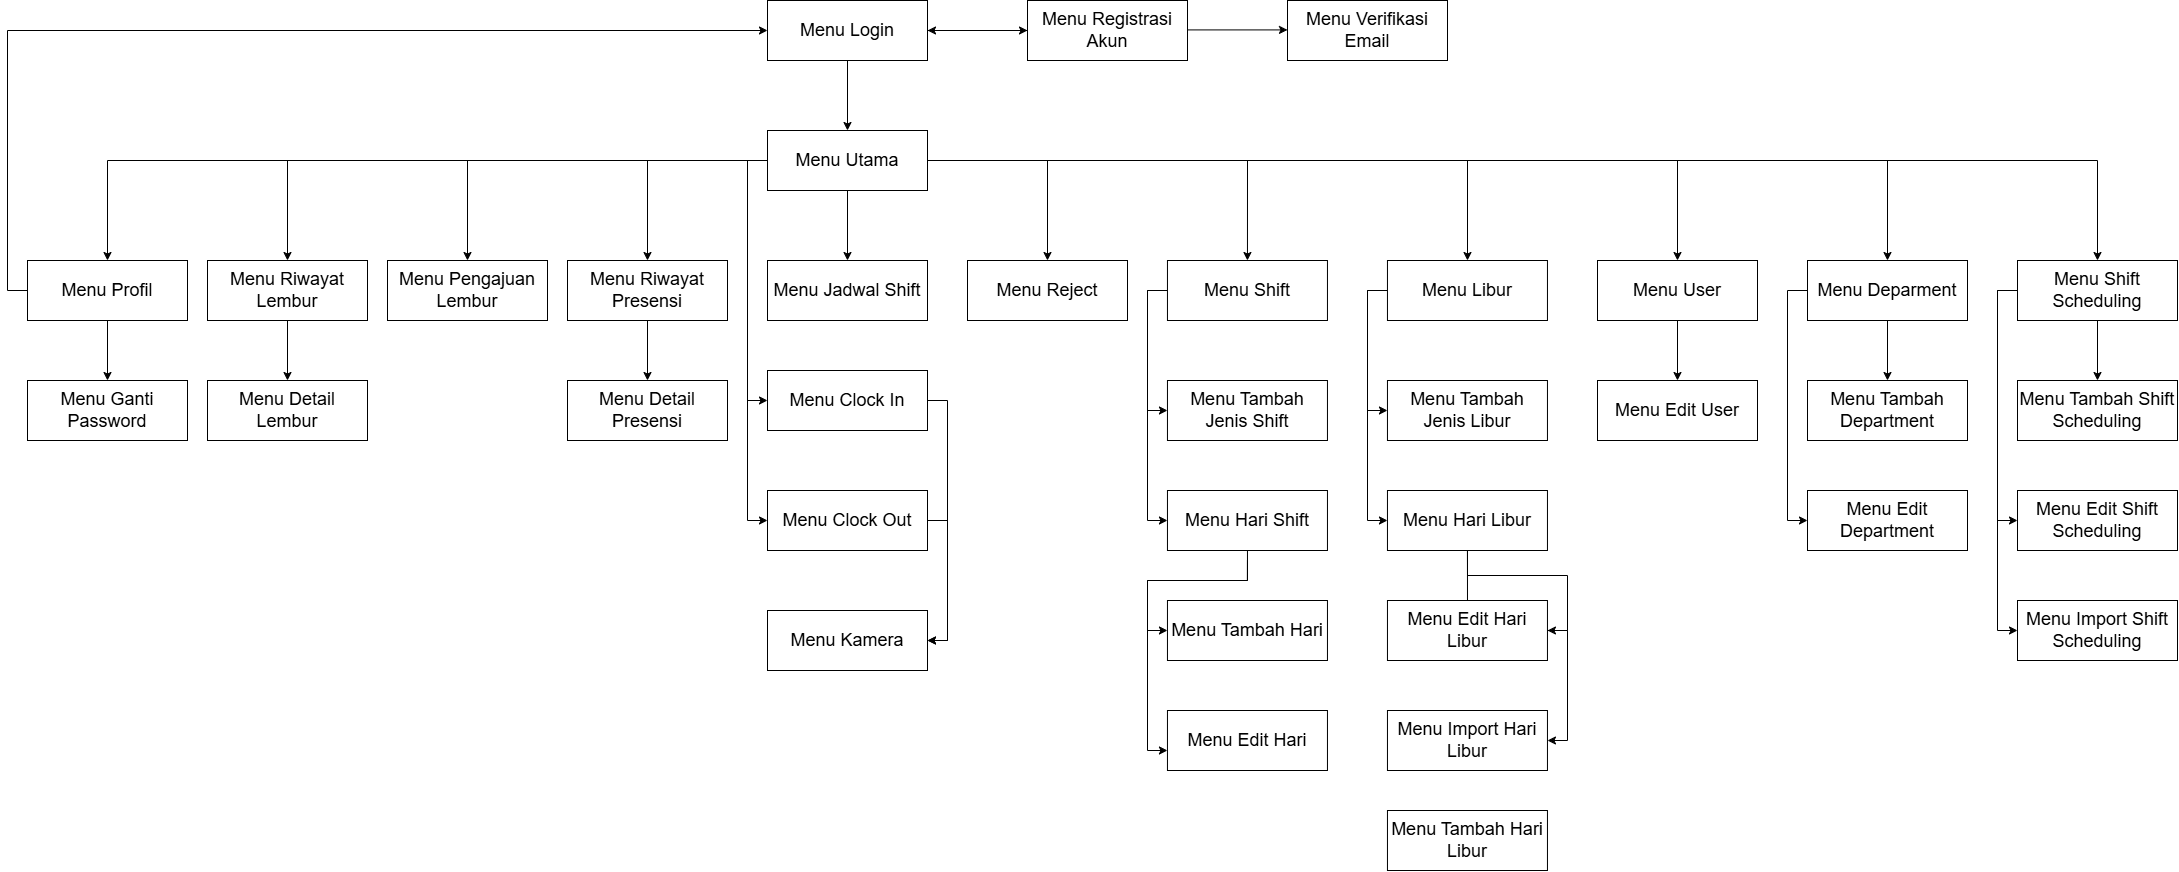
\includegraphics[width=15cm]{Gambar/bab2/windows-navigation-diagram.png}
	\caption{\textit{Windows Navigation Diagram} Aplikasi Presensi \textit{Online}}
	\label{fig:windows-navigation-diagram-aplikasi-presensi-online}
\end{figure}
\FloatBarrier

Pada aplikasi presensi \textit{online} terdiri dari 36 menu yaitu.
\begin{enumerate}
    \item Menu \textit{Utama}
    \\ Menu Utama adalah menu pertama yang muncul saat pengguna membuka aplikasi melalui tautan URL di \textit{website}. Halaman ini hanya dapat diakses ketika pengguna sudah \textit{login} sebelumnya, jika pengguna belum \textit{login} maka akan mengalihkan halaman ke Menu \textit{Login}. Menu ini juga digunakan oleh \textit{staff Infrastructure} untuk melakukan presensi. Tampilan Menu Utama dapat dilihat pada \textbf{\hyperref[sec:mockup-aplikasi-presensi-online]{Lampiran~XI}, \ref{fig:mockup-menu-utama}}.
    
    \item Menu \textit{Login}
    \\ Menu \textit{Login} merupakan menu yang berisi \textit{input form} untuk \textit{login} seluruh pengguna. Jika pengguna sudah \textit{login} sebelumnya maka halaman akan langsung dialihkan ke Menu Utama. Tampilan \textit{mockup} Menu \textit{Login} dapat dilihat pada \textbf{\hyperref[sec:mockup-aplikasi-presensi-online]{Lampiran~XI}, \ref{fig:mockup-menu-login}}.

    \item Menu Registrasi Akun
    \\ Menu Registrasi Akun merupakan halaman yang berisi \textit{input form} yang dapat digunakan oleh pengguna untuk membuat akun baru. Setelah pengguna mendaftar maka tinggal menunggu pengaktifan akun oleh \textit{manager}. Tampilan \textit{mockup} Menu Registrasi Akun dapat dilihat pada \textbf{\hyperref[sec:mockup-aplikasi-presensi-online]{Lampiran~XI}, \ref{fig:mockup-menu-registrasi-akun}}.

    \item Menu Verifikasi \textit{Email}
    \\ Menu Verifikasi \textit{Email} merupakan halaman menu yang menampilkan \textit{input form} kode OTP agar pengguna dapat melakukan verifikasi \textit{email} yang dikirimkan sistem setelah registrasi akun. Tampilan \textit{mockup} Menu Verifikasi \textit{Email} dapat dilihat pada \textbf{\hyperref[sec:mockup-aplikasi-presensi-online]{Lampiran~XI}, \ref{fig:mockup-menu-verifikasi-email}}.

    \item Menu Ganti Password
    \\ Menu Ganti Password merupakan halaman yang berisi \textit{input form} yang dapat digunakan oleh semua pengguna untuk membuat password baru akun. Tampilan \textit{mockup} Menu Ganti Password dapat dilihat pada \textbf{\hyperref[sec:mockup-aplikasi-presensi-online]{Lampiran~XI}, \ref{fig:mockup-menu-ganti-password}}.

    \item Menu Jadwal \textit{Shift}
    \\ Menu Jadwal \textit{Shift} merupakan halaman yang digunakan oleh \textit{staff Infrastructure} untuk melihat \textit{list} jadwal hari dan waktu \textit{shift} kerja. Tampilan \textit{mockup} Menu Jadwal \textit{Shift} dapat dilihat pada \textbf{\hyperref[sec:mockup-aplikasi-presensi-online]{Lampiran~XI}, \ref{fig:mockup-menu-jadwal-shift}}.

    \item Menu \textit{Clock In}
    \\ Menu \textit{Clock In} adalah halaman menu yang digunakan oleh \textit{staff Infrastructure} untuk melakukan presensi masuk. Menu ini dapat diakses ketika \textit{staff Infrastructure} menekan tombol \textit{clock in} pada Menu Utama. Pada menu ini terdapat tombol yang digunakan untuk mengambil lokasi dan tombol untuk menampilkan Menu Kamera. Tampilan \textit{mockup} Menu \textit{Clock In} dapat dilihat pada \textbf{\hyperref[sec:mockup-aplikasi-presensi-online]{Lampiran~XI}, \ref{fig:mockup-menu-clock-in}}.

    \item Menu \textit{Clock Out}
    \\ Menu \textit{Clock Out} adalah halaman menu yang digunakan oleh \textit{staff Infrastructure} untuk melakukan presensi keluar. Pada menu ini terdapat tombol untuk mengambil lokasi dan tombol untuk menampilkan Menu Kamera. Pada saat \textit{staff Infrastructure} melakukan \textit{clock out}, sistem akan mengecek data presensi saat \textit{clock in} dan \textit{clock out}, kemudian secara otomatis membuat data lembur jika presensi dilakukan diluar jam \textit{shift} atau pada hari libur. Tampilan \textit{mockup} Menu \textit{Clock Out} dapat dilihat pada \textbf{\hyperref[sec:mockup-aplikasi-presensi-online]{Lampiran~XI}, \ref{fig:mockup-menu-clock-out}}.

    \item Menu Kamera
    \\ Menu Kamera adalah menu yang digunakan oleh \textit{staff Infrastructure} untuk melakukan pengambilan foto wajah saat melakukan presensi masuk ataupun keluar. Tampilan \textit{mockup} Menu Kamera dapat dilihat pada \textbf{\hyperref[sec:mockup-aplikasi-presensi-online]{Lampiran~XI}, \ref{fig:mockup-menu-kamera}}.

    \item Menu Profil
    \\ Menu Profil adalah menu yang dapat digunakan oleh semua pengguna untuk melakukan \textit{logout} pada aplikasi dan menampilkan menu ganti password. Tampilan \textit{mockup} Menu Profil dapat dilihat pada \textbf{\hyperref[sec:mockup-aplikasi-presensi-online]{Lampiran~XI}, \ref{fig:mockup-menu-profil}}.

    \item Menu Pengajuan Lembur
    \\ Menu Pengajuan Lembur merupakan menu yang digunakan oleh \textit{staff Infrastructure} untuk membuat \textit{form} baru terkait lembur, jika \textit{staff} tersebut lupa melakukan presensi saat lembur. Tampilan \textit{mockup} Menu Pengajuan Lembur dapat dilihat pada \textbf{\hyperref[sec:mockup-aplikasi-presensi-online]{Lampiran~XI}, \ref{fig:mockup-menu-pengajuan-lembur}}.

    \item Menu Riwayat Presensi
    \\ Menu Riwayat Presensi dapat diakses oleh semua pengguna. Menu ini akan menampilkan \textit{list} data presensi yang telah dilakukan dan pengguna dapat melakukan \textit{filter} data agar dapat mencari data secara spesifik. \textit{Manager} dapat melihat seluruh presensi \textit{staff} dan melakukan \textit{export} data presensi dalam bentuk \textit{Microsoft Excel}, sedangkan \textit{staff} hanya dapat melihat presensi miliknya sendiri. Tampilan \textit{mockup} Menu Riwayat Presensi dapat dilihat pada \textbf{\hyperref[sec:mockup-aplikasi-presensi-online]{Lampiran~XI}, \ref{fig:mockup-menu-riwayat-presensi}}.

    \item Menu Detail Presensi
    \\ Menu Detail Presensi dapat diakses dengan memilih salah satu \textit{list} data presensi pada Menu Riwayat Presensi. Menu Detail Presensi menampilkan informasi lengkap dari suatu data presensi. Tampilan \textit{mockup} Menu Detail Presensi dapat dilihat pada \textbf{\hyperref[sec:mockup-aplikasi-presensi-online]{Lampiran~XI}, \ref{fig:mockup-menu-detail-presensi}}.

    \item Menu Riwayat Lembur
    \\ Menu Riwayat Lembur dapat diakses oleh semua pengguna. Menu ini akan menampilkan semua \textit{list} data lembur dan pengguna dapat melakukan \textit{filter} pada data lembur untuk mencari data yang lebih spesifik. \textit{Manager} dapat melihat semua data lembur dan melakukan \textit{export} data presensi dalam bentuk \textit{Microsoft Excel}, sedangkan \textit{staff} hanya dapat melihat data lembur miliknya sendiri. Tampilan \textit{mockup} Menu Riwayat Lembur dapat dilihat pada \textbf{\hyperref[sec:mockup-aplikasi-presensi-online]{Lampiran~XI}, \ref{fig:mockup-menu-riwayat-lembur}}.

    \item Menu Detail Lembur
    \\ Menu Detail Lembur dapat diakses dengan memilih salah satu \textit{list} data lembur pada Menu Riwayat Lembur. Menu Detail Lembur menampilkan informasi lengkap dari suatu data lembur. Tampilan \textit{mockup} Menu Detail Lembur dapat dilihat pada \textbf{\hyperref[sec:mockup-aplikasi-presensi-online]{Lampiran~XI}, \ref{fig:mockup-menu-detail-lembur}}.

    \item Menu \textit{Reject} Lembur
    \\ Menu \textit{Reject} Lembur merupakan menu yang berfungsi untuk melakukan \textit{reject} pada data lembur yang tidak \textit{valid}. \textit{Manager Infrastructure} juga dapat menggunakan fitur \textit{checkbox} untuk melakukan penolakkan lebih dari 1 data lembur. Tampilan \textit{mockup} Menu \textit{Reject} Lembur dapat dilihat pada \textbf{\hyperref[sec:mockup-aplikasi-presensi-online]{Lampiran~XI}, \ref{fig:mockup-menu-reject-lembur}}.

    \item Menu Libur
    \\ Menu Libur merupakan menu yang menampilkan \textit{list} data jenis libur pada perusahnaan. Pada menu ini juga tersedia tombol untuk membuat jenis libur baru dan mengubah data jenis libur. Data jenis libur hanya dapat dikelola oleh \textit{manager}. Tampilan \textit{mockup} Menu Libur dapat dilihat pada \textbf{\hyperref[sec:mockup-aplikasi-presensi-online]{Lampiran~XI}, \ref{fig:mockup-menu-libur}}.

    \item Menu Tambah Libur
    \\ Menu Tambah Libur merupakan menu yang dapat digunakan oleh \textit{manager} untuk membuat jenis libur baru. Tampilan \textit{mockup} Menu Tambah Libur dapat dilihat pada \textbf{\hyperref[sec:mockup-aplikasi-presensi-online]{Lampiran~XI}, \ref{fig:mockup-menu-tambah-libur}}.
    
    \item Menu Hari Libur
    \\ Menu Libur merupakan menu yang menampilkan \textit{list} data hari libur pada perusahnaan dari jenis libur yang dipilih. Pada menu ini juga tersedia tombol untuk membuat hari libur baru, mengubah data hari libur, dan melakukan \textit{import} data libur melalui API. Data hari libur hanya dapat dikelola oleh \textit{manager}. Tampilan \textit{mockup} Menu Libur dapat dilihat pada \textbf{\hyperref[sec:mockup-aplikasi-presensi-online]{Lampiran~XI}, \ref{fig:mockup-menu-hari-libur}}.

    \item Menu Tambah Hari Libur
    \\ Menu Tambah Hari libur dapat digunakan oleh \textit{manager} untuk menambah data hari libur perusahaan secara manual. Tampilan \textit{mockup} Menu Tambah Hari Libur dapat dilihat pada \textbf{\hyperref[sec:mockup-aplikasi-presensi-online]{Lampiran~XI}, \ref{fig:mockup-menu-tambah-hari-libur}}.

    \item Menu \textit{Edit} Hari Libur
    \\ Menu \textit{Edit} Hari Libur merupakan menu yang digunakan oleh \textit{manager} untuk mengubah data hari libur yang sudah ada. Tampilan \textit{mockup} Menu Hari \textit{Edit} Libur dapat dilihat pada \textbf{\hyperref[sec:mockup-aplikasi-presensi-online]{Lampiran~XI}, \ref{fig:mockup-menu-edit-hari-libur}}.

    \item Menu \textit{Import} Hari Libur
    \\ Menu \textit{Import} Hari Libur merupakan menu yang dapat digunakan oleh \textit{manager} untuk mendapatkan data libur nasional berdasarkan tahun yang dipilih melalui API, kemudian menambahkan data hari libur tersebut ke dalam jenis libur. Tampilan \textit{mockup} Menu \textit{Import} Hari Libur dapat dilihat pada \textbf{\hyperref[sec:mockup-aplikasi-presensi-online]{Lampiran~XI}, \ref{fig:mockup-menu-import-libur}}.

    \item Menu \textit{User}
    \\ Menu \textit{User} adalah menu yang menampilkan data \textit{list user} pada aplikasi presensi \textit{online}. Menu ini digunakan oleh \textit{manager} untuk mengelola data \textit{user}. Tampilan \textit{mockup} Menu \textit{User} dapat dilihat pada \textbf{\hyperref[sec:mockup-aplikasi-presensi-online]{Lampiran~XI}, \ref{fig:mockup-menu-user}}.

    \item Menu \textit{Edit User}
    \\ Menu \textit{Edit User} merupakan menu yang digunakan oleh \textit{manager} untuk mengubah data \textit{user} seperti mengantur \textit{shift} yang digunakan oleh \textit{staff} dan status aktif akun pada \textit{user}. Tampilan \textit{mockup} Menu \textit{Edit User} dapat dilihat pada \textbf{\hyperref[sec:mockup-aplikasi-presensi-online]{Lampiran~XI}, \ref{fig:mockup-menu-edit-user}}.

    \item Menu \textit{Department}
    \\ Menu \textit{Department} adalah menu yang menampilkan data \textit{list department} pada aplikasi presensi \textit{online}. Menu ini digunakan oleh \textit{manager} untuk mengelola data \textit{department}. Tampilan \textit{mockup} Menu \textit{Department} dapat dilihat pada \textbf{\hyperref[sec:mockup-aplikasi-presensi-online]{Lampiran~XI}, \ref{fig:mockup-menu-department}}.

    \item Menu Tambah \textit{Department}
    \\ Menu Tambah \textit{Department} merupakan menu yang digunakan oleh \textit{manager} untuk menambah data \textit{department} baru. Tampilan \textit{mockup} Menu Tambah \textit{Department} dapat dilihat pada \textbf{\hyperref[sec:mockup-aplikasi-presensi-online]{Lampiran~XI}, \ref{fig:mockup-menu-tambah-department}}.

    \item Menu \textit{Edit Department}
    \\ Menu \textit{Edit Department} merupakan menu yang digunakan oleh \textit{manager} untuk mengubah data \textit{department}. Tampilan \textit{mockup} Menu \textit{Edit Department} dapat dilihat pada \textbf{\hyperref[sec:mockup-aplikasi-presensi-online]{Lampiran~XI}, \ref{fig:mockup-menu-edit-department}}.

    \item Menu \textit{Shift}
    \\ Menu \textit{Shift} merupakan menu yang menampilkan \textit{list shift} yang telah dibuat. Menu ini berfungsi untuk mengelola data jenis \textit{shift} oleh \textit{manager}. Tampilan \textit{mockup} Menu \textit{Shift} dapat dilihat pada \textbf{\hyperref[sec:mockup-aplikasi-presensi-online]{Lampiran~XI}, \ref{fig:mockup-menu-shift}}. 

    \item Menu Tambah \textit{Shift}
    \\ Menu Tambah \textit{Shift} adalah menu yang dapat digunakan oleh \textit{manager} untuk menambahkan jenis \textit{shift} baru. Tampilan \textit{mockup} Menu Tambah \textit{Shift} dapat dilihat pada \textbf{\hyperref[sec:mockup-aplikasi-presensi-online]{Lampiran~XI}, \ref{fig:mockup-menu-tambah-shift}}.

    \item Menu Hari \textit{Shift}
    \\ Menu Hari \textit{Shift} merupakan menu yang berfungsi untuk mengubah nama jenis \textit{shift} dan mengelola hari dan waktu pada jenis \textit{shift} yang dipilih oleh \textit{manager}. Tampilan \textit{mockup} Menu Hari \textit{Shift} dapat dilihat pada \textbf{\hyperref[sec:mockup-aplikasi-presensi-online]{Lampiran~XI}, \ref{fig:mockup-menu-edit-shift}}.

    \item Menu Tambah Hari \textit{Shift}
    \\ Menu Tambah Hari \textit{Shift} adalah menu yang berisi \textit{input form} yang dapat digunakan oleh \textit{manager} untuk menambah hari dan waktu pada jenis \textit{shift} yang sedang di-\textit{edit}. Tampilan \textit{mockup} Menu Tambah Hari \textit{Shift} dapat dilihat pada \textbf{\hyperref[sec:mockup-aplikasi-presensi-online]{Lampiran~XI}, \ref{fig:mockup-menu-tambah-hari}}.

    \item Menu \textit{Edit} Hari \textit{Shift}
    \\ Menu \textit{Edit} Hari \textit{Shift} merupakan menu yang berisi \textit{input form} yang digunakan oleh \textit{manager} untuk mengubah hari dan waktu pada jenis \textit{shift} yang dipilih. Tampilan \textit{mockup} Menu \textit{Edit} Hari \textit{Shift} dapat dilihat pada \textbf{\hyperref[sec:mockup-aplikasi-presensi-online]{Lampiran~XI}, \ref{fig:mockup-menu-edit-hari}}.

    \item Menu \textit{Shift Scheduling}
    \\ Menu \textit{Shift Scheduling} adalah menu yang didapat digunakan oleh \textit{manager} untuk melihat \textit{list} penjadwalan \textit{shift} yang akan dipakai setiap \textit{staff} berdasarkan kurun waktu tertentu dan dapat meng-\textit{export} seluruh data penjadwalan menjadi format \textit{Excel}. Tampilan \textit{mockup} Menu \textit{Shift Scheduling} dapat dilihat pada \textbf{\hyperref[sec:mockup-aplikasi-presensi-online]{Lampiran~XI}, \ref{fig:mockup-menu-scheduling-shift}}.

    \item Menu Tambah \textit{Shift Scheduling}
    \\ Menu \textit{Shift Scheduling} adalah menu yang didapat digunakan oleh \textit{manager} untuk membuat penjadwalan \textit{shift} pada \textit{staff} dengan kurun waktu yang dipilih. Tampilan \textit{mockup} Menu Tambah \textit{Shift Scheduling} dapat dilihat pada \textbf{\hyperref[sec:mockup-aplikasi-presensi-online]{Lampiran~XI}, \ref{fig:mockup-menu-tambah-scheduling-shift}}.

    \item Menu \textit{Edit} \textit{Shift Scheduling}
    \\ Menu \textit{Edit Shift Scheduling} adalah menu yang didapat digunakan oleh \textit{manager} untuk mengubah data penjadwalan \textit{shift} pada \textit{staff} yang sudah ada. Tampilan \textit{mockup} Menu \textit{Edit} \textit{Shift Scheduling} dapat dilihat pada \textbf{\hyperref[sec:mockup-aplikasi-presensi-online]{Lampiran~XI}, \ref{fig:mockup-menu-edit-scheduling-shift}}.

    \item Menu \textit{Import} \textit{Shift Scheduling}
    \\ Menu \textit{Import Shift Scheduling} adalah menu yang didapat digunakan oleh \textit{manager} untuk meng-\textit{upload} \textit{file Excel} yang berisi \textit{list} jadwal \textit{shift} yang akan digunakan oleh setiap \textit{staff}. Tampilan \textit{mockup} Menu \textit{Import} \textit{Shift Scheduling} dapat dilihat pada \textbf{\hyperref[sec:mockup-aplikasi-presensi-online]{Lampiran~XI}, \ref{fig:mockup-menu-import-scheduling-shift}}.

    

    \end{enumerate}

\section{Perancangan Pembuatan Kode}
\label{sec:perancangan-pembuatan-kode}
\subsection{Teori}
Pada bagian teori akan menjelaskan tentang bahasa pemrograman, \textit{framework}, \textit{library}, dan basis data yang akan digunakan pada skripsi ini.

\subsubsection{HTML}
HTML adalah bahasa komputer yang dirancang khusus untuk membuat situs web yang dapat diakses oleh siapa saja tanpa memandang lokasi atau zona waktu. HTML merupakan singkatan dari \textit{Hyper Text Markup Language}. Hyper Text adalah metode yang digunakan untuk berpindah di internet~\cite{html2017micheal}. Pada dasarnya, HTML tidak lebih dari sekumpulan kode \textit{markup} yang disebut elemen yang menentukan struktur halaman web~\cite{html2024paul}. HTML memungkinkan pengembangan situs web yang dapat diakses di berbagai jenis perangkat, mulai dari PC hingga \textit{smartphone}, tanpa memerlukan instalasi \textit{plugin} yang berulang pada \textit{browser} atau pengembangan beberapa versi situs web khusus untuk perangkat seluler~\cite{theabsolute2023kevin}. Contoh kode HTML dapat dilihat pada \textbf{\ref{fig:kode-html}}.

\subsubsection{CSS}
CSS (\textit{Cascading Style Sheet}) adalah bahasa stylesheet yang diterapkan untuk menentukan bagaimana elemen HTML ditampilkan pada halaman web, termasuk desain, tata letak, dan variasi untuk perangkat dengan ukuran layar yang berbeda. CSS mengelola tata letak dari banyak situs web secara bersamaan~\cite{html2023sufyan}. CSS adalah alat yang unik dalam pengembangan perangkat lunak. Meskipun bukan bahasa pemrograman dalam arti tradisional, CSS tetap membutuhkan pemikiran abstrak~\cite{css2023keith}. CSS memberikan fleksibilitas dalam desain web, memungkinkan konsistensi di seluruh situs sekaligus memudahkan perubahan pada halaman individu atau bagian tertentu sesuai kebutuhan~\cite{mastering2023sufyan}. Contoh kode CSS dapat dilihat pada \textbf{\ref{fig:kode-css}}.

%%%%%%%%%%%%%%%%%%%%%%%%%%%%%%%%%%%%%%%%%%%%%%%%
\begin{figure}[!htbp]
	\centering
	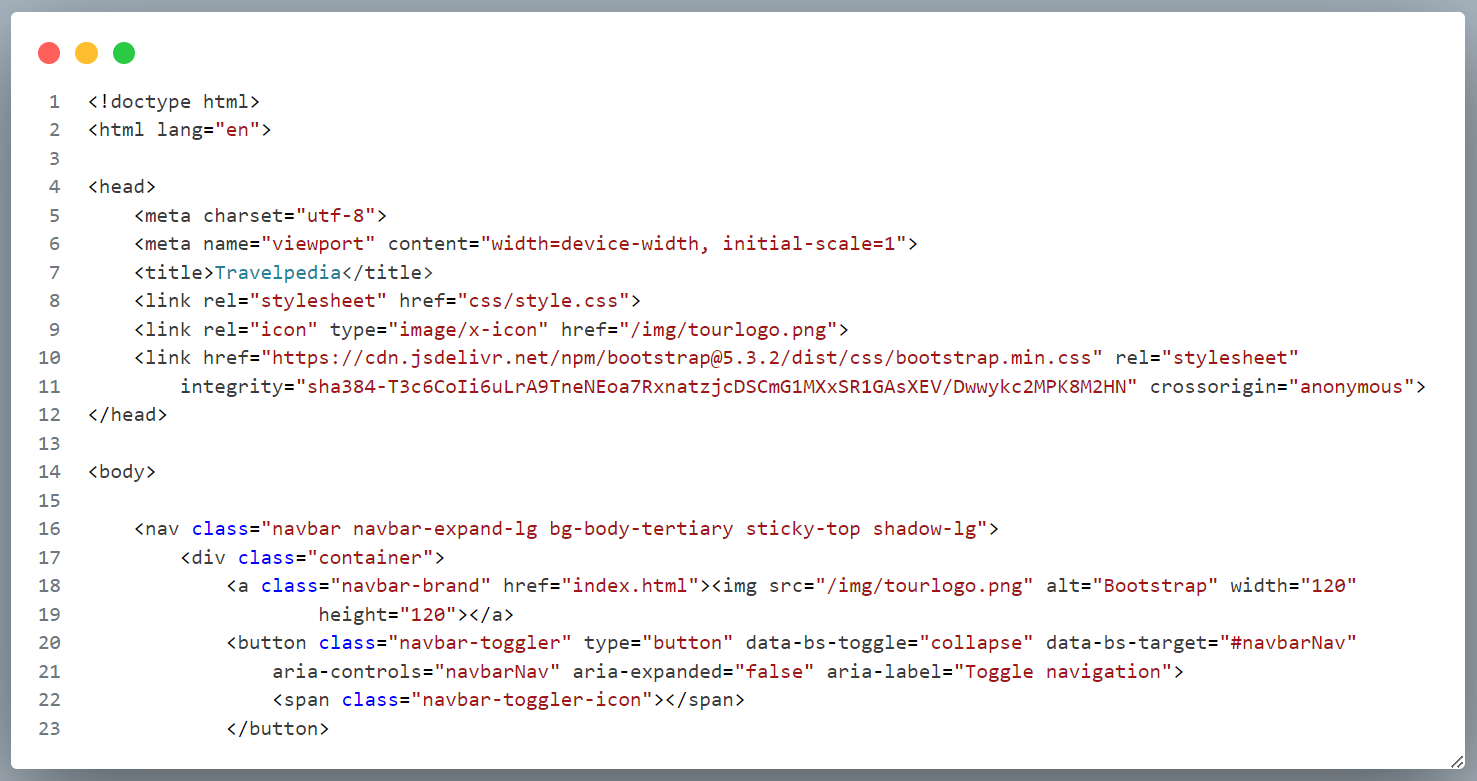
\includegraphics[width=16cm]{Gambar/bab2/html.png}
	\caption{Kode HTML}
	\label{fig:kode-html}
\end{figure}
\FloatBarrier

%%%%%%%%%%%%%%%%%%%%%%%%%%%%%%%%%%%%%%%%%%%%%%%%
\begin{figure}[!htbp]
	\centering
	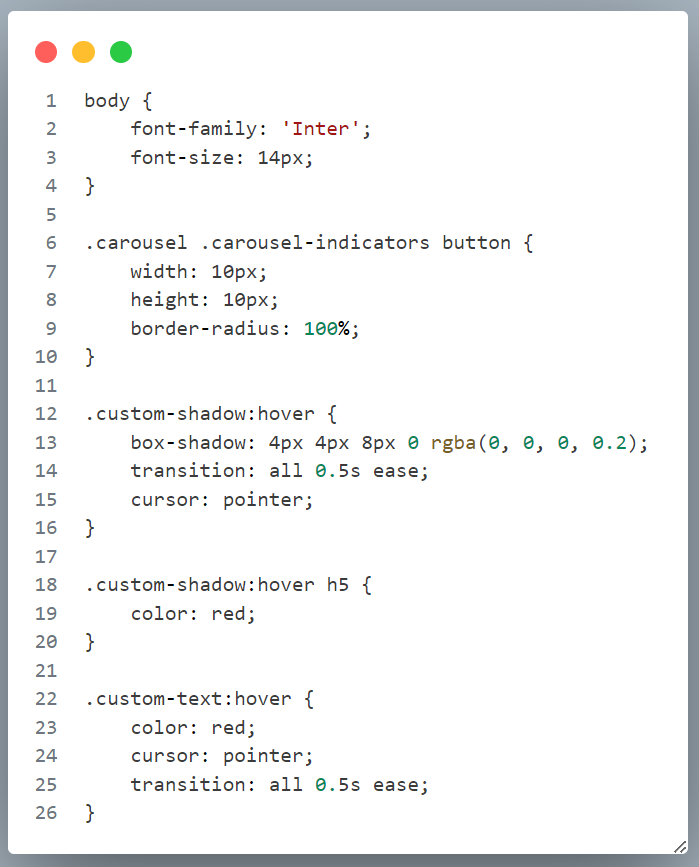
\includegraphics[width=7cm]{Gambar/bab2/css.png}
	\caption{Kode CSS}
	\label{fig:kode-css}
\end{figure}
\FloatBarrier

\subsubsection{JavaScript}
JavaScript adalah bahasa pemrograman dinamis yang terutama digunakan untuk membuat elemen interaktif pada halaman web. JavaScript memungkinkan pengembang untuk menambahkan berbagai fungsionalitas ke halaman web, termasuk validasi formulir, peta interaktif, grafik animasi, dan tata letak halaman web yang kompleks. Tidak seperti banyak bahasa pemrograman lainnya, JavaScript dieksekusi di browser pengguna (\textit{client-side})~\cite{basics2024unknown}. Dalam JavaScript, terdapat teknik bernama ajax yang berfungsi untuk membuat permintaan ke server untuk data tambahan tanpa perlu memuat ulang halaman web, yang menghasilkan pengalaman pengguna yang lebih baik~\cite{professional2023matt}. HTML DOM (\textit{Document Object Model}) merepresentasikan segala sesuatu di halaman HTML sebagai sebuah pohon Node, termasuk komentar HTML dan setiap spasi kosong. Semua elemen dalam DOM dapat diakses oleh JavaScript dan bisa diubah, dan setiap perubahan yang dilakukan oleh JavaScript akan langsung tercermin di halaman yang ditampilkan kepada pengguna~\cite{quick2023david}. Contoh kode JavaScript dapat dilihat pada \textbf{\ref{fig:kode-javascript}}.
%%%%%%%%%%%%%%%%%%%%%%%%%%%%%%%%%%%%%%%%%%%%%%%%
\begin{figure}[!htbp]
	\centering
	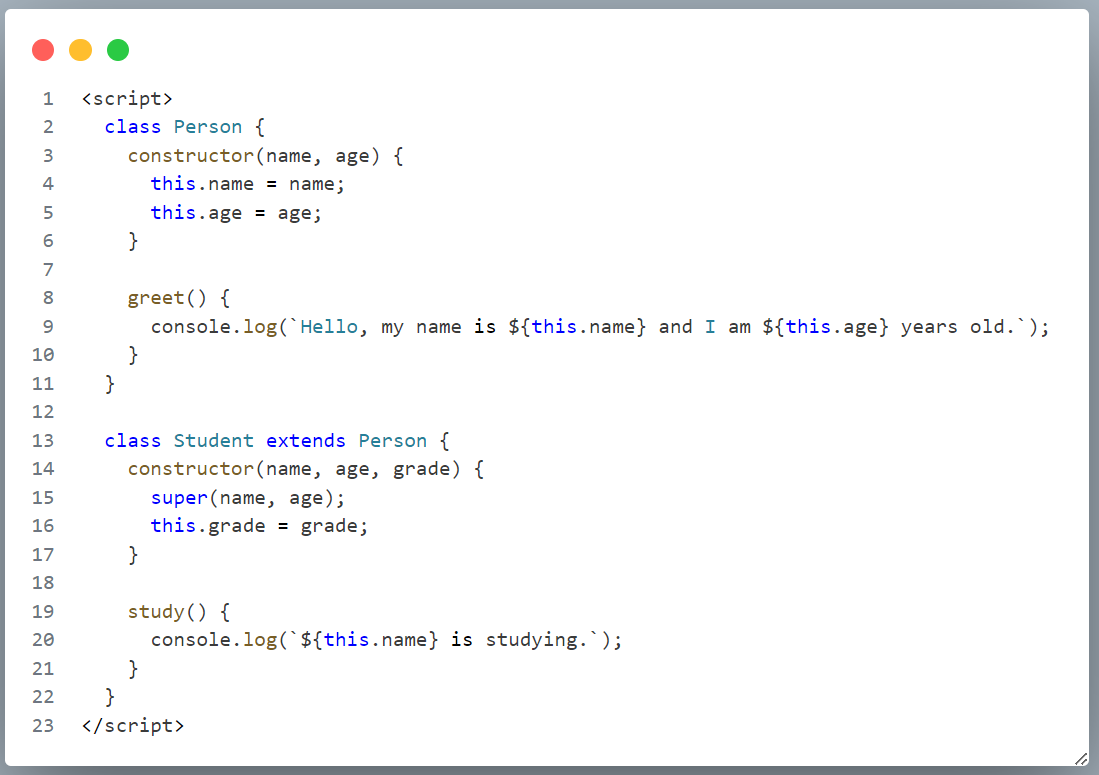
\includegraphics[width=14cm]{Gambar/bab2/javascript.png}
	\caption{Kode JavaScript}
	\label{fig:kode-javascript}
\end{figure}
\FloatBarrier

\subsubsection{PHP}
PHP adalah bahasa pemrograman yang berjalan di sisi server, berbeda dengan JavaScript yang merupakan bahasa pemrograman sisi klien~\cite{php2022tom}. PHP mendukung berbagai \textit{database} populer, seperti MySQL, PostgreSQL, Oracle, Sybase, Informix, dan \textit{Microsoft} SQL \textit{Server}, yang membuatnya fleksibel untuk berbagai kebutuhan pengembangan aplikasi web~\cite{php2022sufyan}. Contoh kode PHP dapat dilihat pada \textbf{\ref{fig:kode-php}}.
%%%%%%%%%%%%%%%%%%%%%%%%%%%%%%%%%%%%%%%%%%%%%%%%
\begin{figure}[!htbp]
	\centering
	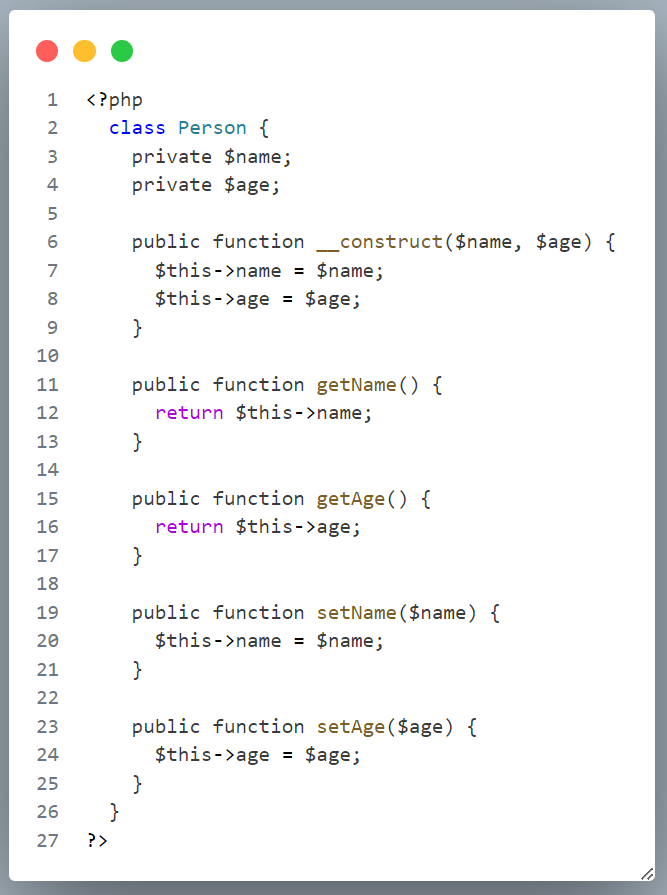
\includegraphics[width=8cm]{Gambar/bab2/php.png}
	\caption{Kode PHP}
	\label{fig:kode-php}
\end{figure}
\FloatBarrier

\subsubsection{JQuery}
jQuery bertujuan untuk menyederhanakan dan meningkatkan efisiensi penggunaan JavaScript dengan membuatnya lebih cepat, mudah, ringkas, dan menarik. \textit{Library} ini memungkinkan pengembang untuk membuat situs web yang lebih dinamis dan interaktif dengan memanfaatkan berbagai metode bawaan yang telah ditentukan. Dengan jQuery, banyak fungsi JavaScript yang biasa digunakan, yang biasanya memerlukan beberapa baris kode, dapat diakses dan dijalankan hanya dengan satu baris kode, sehingga mempercepat dan mempermudah proses pengembangan~\cite{masteringjquery2023sufyan}. Dokumentasi JQuery dapat diakses melalui \url{https://api.jquery.com/}. Contoh kode JQuery dapat dilihat pada \textbf{\ref{fig:kode-jquery}}.
%%%%%%%%%%%%%%%%%%%%%%%%%%%%%%%%%%%%%%%%%%%%%%%%
\begin{figure}[!htbp]
	\centering
	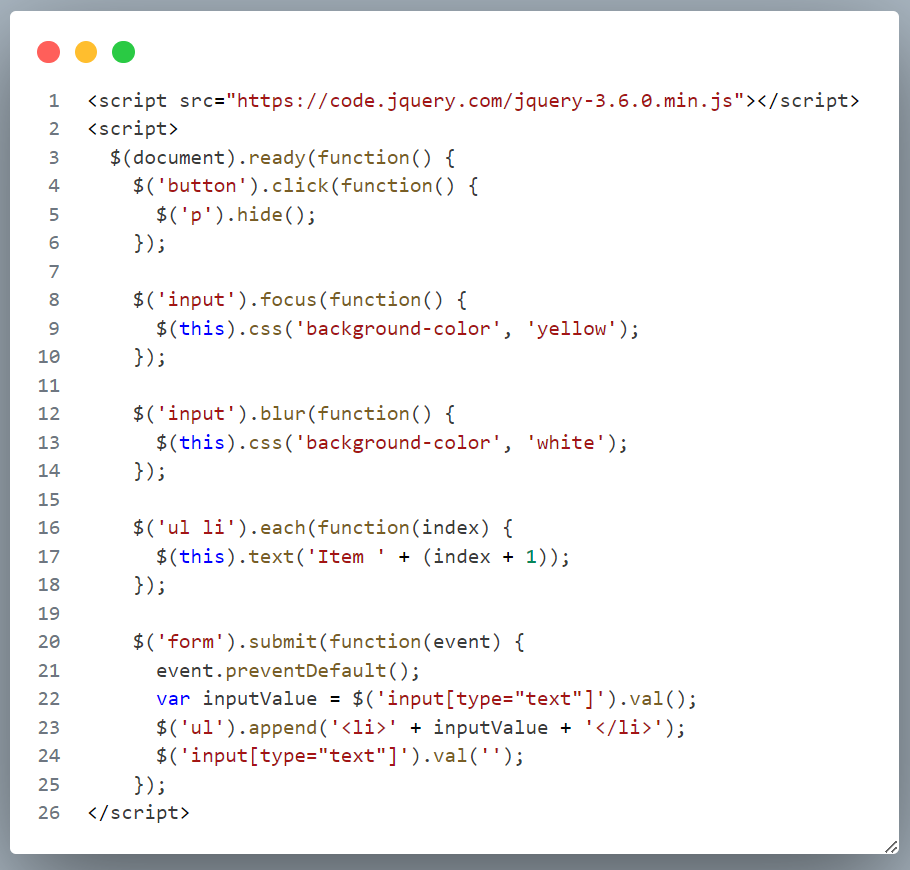
\includegraphics[width=10cm]{Gambar/bab2/jquery.png}
	\caption{Kode JQuery}
	\label{fig:kode-jquery}
\end{figure}
\FloatBarrier

\subsubsection{Laravel}
Laravel adalah \textit{framework} PHP yang gratis dan sumber terbuka yang menyediakan seperangkat alat dan sumber daya untuk membangun aplikasi web PHP modern. Laravel menyediakan sintaks yang elegan, fitur bawaan, dan berbagai paket serta ekstensi yang kompatibel. Saat pengembangan Laravel secara \textit{local}, membutuhkan XAMPP dan \textit{composer}. XAMPP adalah lingkungan pengembangan PHP yang paling populer. XAMPP adalah distribusi Apache yang gratis dan mudah diinstal yang mencakup MySQL, PHP, dan Perl. Composer adalah alat untuk mengelola ketergantungan dalam pengembangan PHP. Alat ini memudahkan mengelola \textit{libraries} yang dibutuhkan saat pengembangan proyek~\cite{practical2022daniel}. \textit{Framework} ini menyederhanakan berbagai tugas umum dalam pengembangan web, seperti interaksi dengan \textit{database}, autentikasi, antrian, pengiriman \textit{email}, dan \textit{caching}, berkat komponen-komponennya yang terintegrasi~\cite{laravel2023matt}. Dokumentasi Laravel dapat diakses melalui \url{https://laravel.com/docs/10.x/installation}. Kode \textit{command line} untuk instalasi \textit{framework} Laravel dengan composer dapat dilihat pada \textbf{\ref{fig:install-laravel}}. 
%%%%%%%%%%%%%%%%%%%%%%%%%%%%%%%%%%%%%%%%%%%%%%%%
\begin{figure}[!htbp]
	\centering
	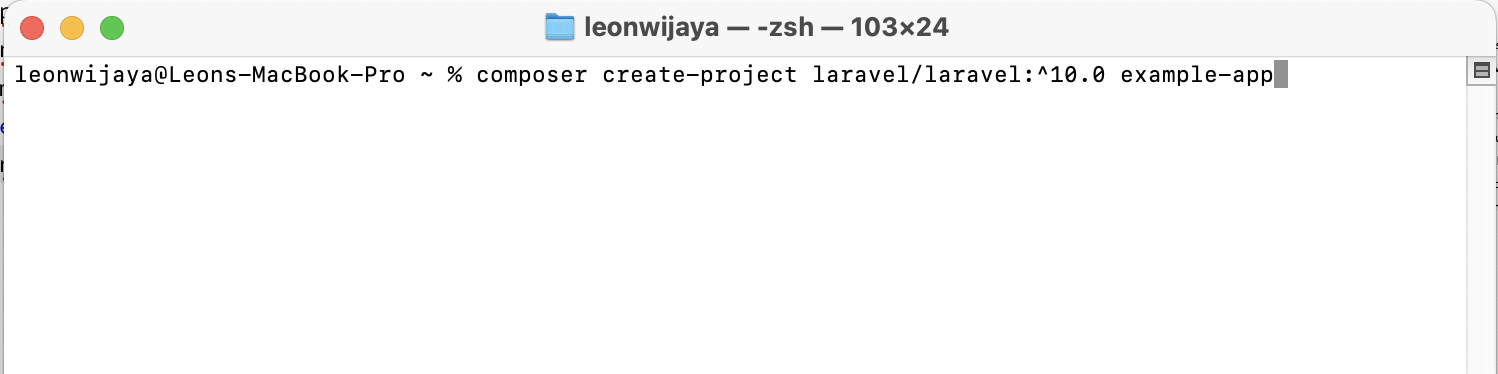
\includegraphics[width=8cm]{Gambar/bab2/install-laravel.png}
	\caption{Kode \textit{Command Line} Instalasi \textit{Framework} Laravel dengan Composer}
	\label{fig:install-laravel}
\end{figure}
\FloatBarrier

\subsubsection{TensorFlow}
TensorFlow adalah \textit{framework machine learning} yang memungkinkan pengembang untuk mengembangkan solusi \textit{machine learning} dengan cepat untuk berbagai kasus penggunaan khusus yang dapat memanfaatkan  \textit{machine learning}~\cite{thushan2022tensorflow}. TensorFlow dibuat di Google dan mendukung banyak aplikasi  \textit{machine learning} skala besar~\cite{hands2022aurelien}. TensorFlow memungkinkan pengembang untuk mendefinisikan dan melatih berbagai jenis model \textit{machine learning}, termasuk \textit{deep neural networks}, untuk berbagai tugas seperti \textit{classification}, \textit{regression}, \textit{clustering}, dan lain-lain~\cite{mastering2024hasan}. Pada aplikasi ini, model \textit{simple face detection (BlazeFace)} akan digunakan untuk mendeteksi wajah pada gambar selama pengambilan foto saat melakukan presensi. Dokumentasi TensorFlow dapat dilihat melalui \url{https://www.tensorflow.org/js/models}.

\subsubsection{Tailwind CSS}
Tailwind adalah sekumpulan kelas utilitas dasar yang dapat digunakan seperti blok penyusun untuk menciptakan berbagai desain yang kita inginkan. \textit{Framework} yang berfokus pada utilitas ini mencakup properti CSS yang paling penting, tetapi juga mudah diperluas dengan berbagai cara~\cite{tailwind2022ivaylo}. Tailwind CSS memiliki beberapa keunggulan, termasuk kemudahan dalam membuat prototipe, iterasi, dan kustomisasi tampilan, serta menyediakan \textit{modifier} untuk perilaku khusus. Selain itu, penggunaan Tailwind mengurangi penulisan CSS karena desain lebih banyak berasal dari komposisi \textit{utility}-nya~\cite{modern2022noel}. Dokumentasi Tailwind CSS dapat diakses melalui \url{https://tailwindcss.com/docs/installation}. Penulis menggunakan Tailwind CSS sebagai alat untuk mempermudah proses \textit{styling} pada tampilan aplikasi.


\subsubsection{Flowbite}
Flowbite merupakan \textit{library} komponen UI \textit{open source} yang dikembangakan dengan \textit{framework} Tailwind CSS yang berfokus pada pendekatan \textit{utility first}. \textit{Library} ini menyediakan berbagai komponen penting yang sering digunakan dalam pengembangan web, seperti tombol, \textit{dropdown}, \textit{navigation bar}, dan \textit{modal}~\cite{introduction2024flowbite}. Dokumentasi Flowbite dapat diakses melalui \url{https://flowbite.com/docs/getting-started/introduction/}. Penulis menggunakan Flowbite untuk mempercepat proses pembuata antarmuka pengguna (UI) karena terdapat komponen siap pakai.

\subsubsection{MySQL}
MySQL adalah sistem manajemen basis data relasional (RDBMS) sumber terbuka yang dikembangkan oleh perusahaan Swedia, MySQL AB. Perusahaan ini didirikan oleh David Axmark, Allan Larsson, dan Michael Widenius, dengan pengembangan awal MySQL dimulai oleh Widenius dan Axmark pada tahun 1994~\cite{masteringmysql2022sufyan}. MySQL banyak digunakan oleh beberapa organisasi dan pengembang karena beberapa alasan utama diantaranya yaitu bersifat open-source dan biasanya gratis, kinerja yang sangat cepat, mudah di-\textit{install} dan digunakan~\cite{mysql2023ben}.
